\RequirePackage{luatex85}
\documentclass{standalone}

\usepackage{fontspec, unicode-math}
\setsansfont[Scale=MatchLowercase]{TeX Gyre Heros}
\setmathfont{TeX Gyre Termes Math}

\usepackage{tikz}
\usetikzlibrary{matrix}

\tikzset{
  every picture/.style={font={\sffamily\normalsize}, >=stealth},
  every pin edge/.style={black}}

\begin{document}

  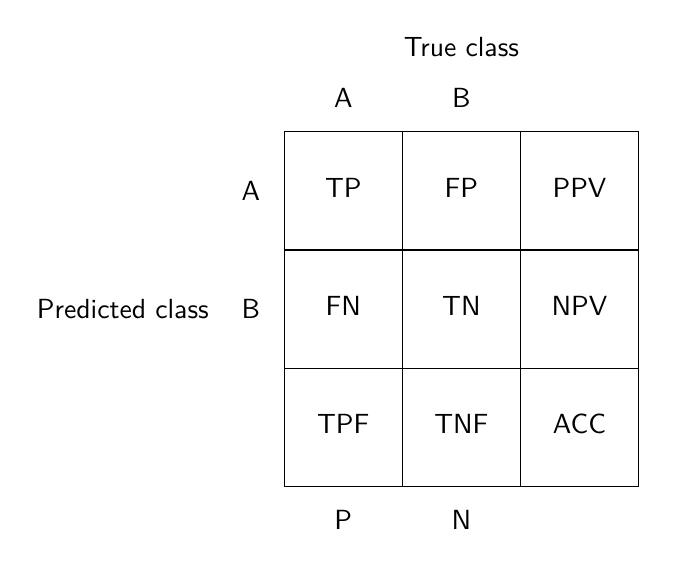
\begin{tikzpicture}[
    confusionmatrix/.style={
      matrix of nodes,
      nodes in empty cells,
      column sep = -\pgflinewidth,
      row sep = -\pgflinewidth,
      nodes={
        draw,
        minimum size=1.5cm,
        text height=\ht\strutbox,
        text depth=\dp\strutbox}}]

    \matrix[confusionmatrix] (confusionmatrix) {
       \node (TP) {TP};   & \node (FP) {FP};   & PPV \\
       \node (FN) {FN};   & TN                 & NPV \\
       \node (TPF) {TPF}; & \node (TNF) {TNF}; & ACC \\
    };

    \node[above=20pt] at (confusionmatrix.north) {True class};
    \node[align=center, left=20pt] at (confusionmatrix.west) {Predicted class};

    \node[above=5pt] at (TP.north) {A};
    \node[above=5pt] at (FP.north) {B};

    \node[left=5pt] at (TP.west) {A};
    \node[left=5pt] at (FN.west) {B};    

    \node[below=5pt] at (TPF.south) {P};
    \node[below=5pt] at (TNF.south) {N};
  \end{tikzpicture}

\end{document}
